\documentclass[conference]{IEEEtran}
\IEEEoverridecommandlockouts
% The preceding line is only needed to identify funding in the first footnote. If that is unneeded, please comment it out.
\usepackage{cite}
\usepackage{amsmath,amssymb,amsfonts}
\usepackage{algorithmic}
\usepackage{graphicx}
\usepackage{textcomp}
\usepackage{hyperref}
\usepackage{xcolor}
\usepackage{booktabs}
\usepackage{multirow}
\def\BibTeX{{\rm B\kern-.05em{\sc i\kern-.025em b}\kern-.08em
    T\kern-.1667em\lower.7ex\hbox{E}\kern-.125emX}}
\graphicspath{{Images/}{./}} 

\begin{document}

\title{Estimation of Vehicle Mass and Road Grade\\
{\footnotesize \large CS116.O11.KHCL - Machine Learning with Python: Final Project}
}

\author{\IEEEauthorblockN{Nguyen Hoang Tan} 
\IEEEauthorblockA{\textit{MSSV: 215214113} \\
21521413@gm.uit.edu.vn}
}

\maketitle

\begin{abstract}
    The Estimation of Vehicle Mass and Road Grade is a crucial aspect of modern transportation systems. This report details our approach, encompassing exploratory data analysis (EDA), feature engineering, data splitting, model selection, and evaluation, resulting in achieving the 1st rank in both public and private contest datasets.
\end{abstract}

% \begin{IEEEkeywords}
%     Machine Learning, Vehicle Mass Estimation, Road Grade Estimation, Sensor Data, Supervised Learning, Feature Engineering.
% \end{IEEEkeywords}

\section{Introduction}
The Estimation of Vehicle Mass and Road Grade is a multifaceted challenge within the domain of transportation engineering, encompassing critical aspects such as fuel efficiency, vehicle performance, and overall safety. This project leverages machine learning methodologies to address this complex problem. We employ \href{https://scikit-learn.org/stable/modules/generated/sklearn.ensemble.RandomForestClassifier.html}{\textbf{Random Forest Classifier}} for Vehicle Mass and \href{https://scikit-learn.org/stable/modules/generated/sklearn.neighbors.KNeighborsRegressor.html}{\textbf{K-Nearest Neighbors Regressor}} for Road Grade estimation, focusing on the utilization of diverse signals collected from a vehicle to predict both its mass and the grade of the road it traverses.

\section{Dataset Description}
The dataset used in this project comprises eleven signals obtained from a vehicle, with the first nine serving as input features, and the last two as output variables. Notably, the data lacks time information, and the order of recordings has been deliberately scrambled. Each record in the dataset represents an individual frame, and the absence of temporal information necessitates an algorithmic approach that operates independently on each frame.

The signals include key parameters such as engine speed, vehicle speed, torque-related metrics, clutch and engine operation status, as well as the desired torque or torque limit. Of particular significance are the signals indicating road slope and the vehicle's mass, represented as either 38 t or 49 t.


\section{Exploratory Data Analysis (EDA)}
Before delving into the machine learning models, it is crucial to conduct an Exploratory Data Analysis (EDA) to gain insights into the dataset's characteristics and identify potential patterns or anomalies. 

\noindent \textbf{Data Integrity Check} \hspace{0.2em} Checking for missing values. Fortunately, the dataset demonstrates completeness, as no null values are present across any of the features.

\noindent \textbf{Outlier Detection} \hspace{0.2em} Generate box plots for each feature (excluding the target variable, Vehicle\_Mass) to identify potential outliers. 

\begin{figure}[h]
    \centering
    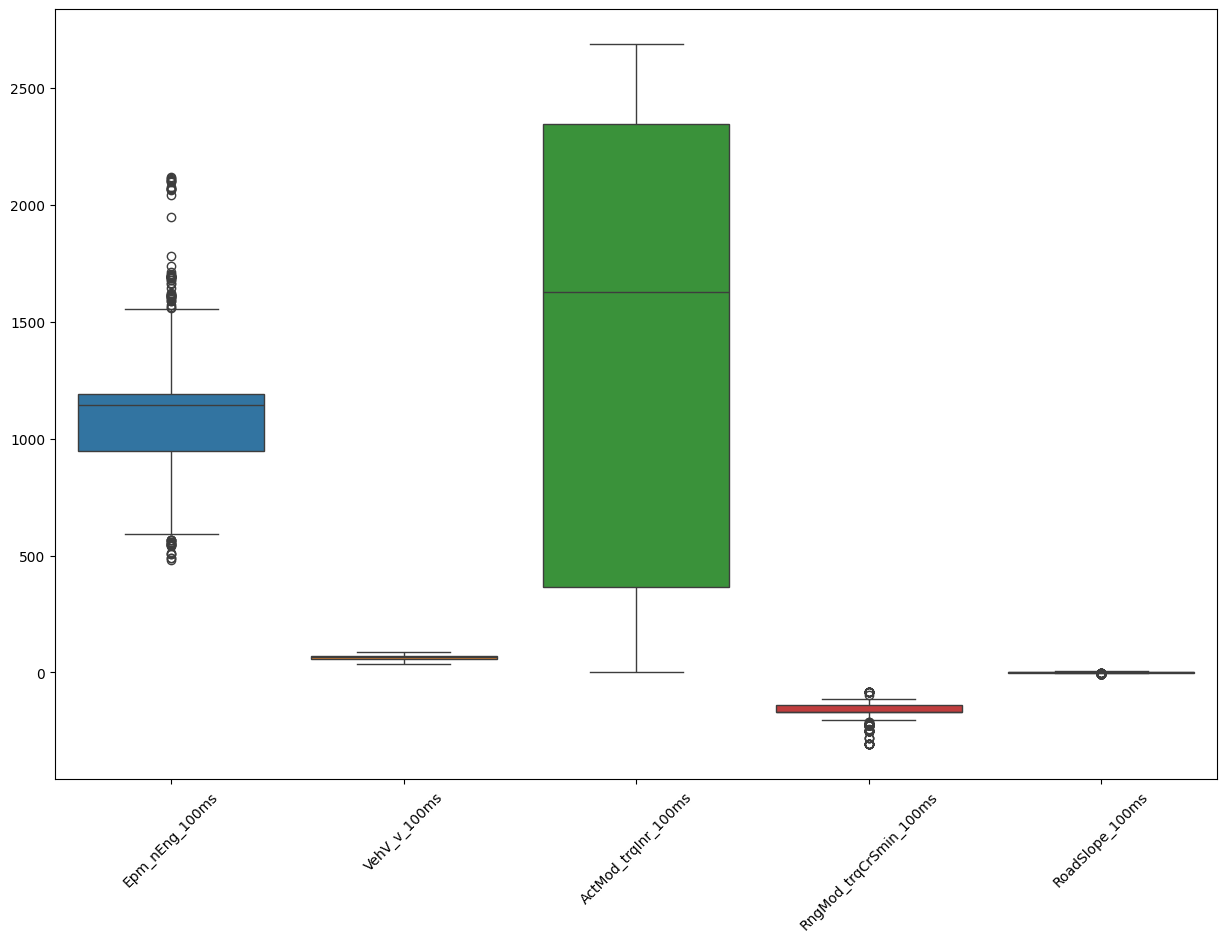
\includegraphics[width=0.5\textwidth]{Boxplot.png}
    \caption{Box Plot of Feature Columns }
    \label{boxplot}
\end{figure}

Figure \ref{boxplot} revealed the presence of numerous outliers across several features, potentially impacting the performance of machine learning models.

To mitigate the influence of outliers, We can utilize the \href{https://scikit-learn.org/stable/modules/generated/sklearn.preprocessing.RobustScaler.html}{\textbf{RobustScaler}} during the feature scaling process. \\

\noindent \textbf{Correlation Analysis} \hspace{0.2em} Table \ref{tab:correlation} provides insights into the relationships between variables, highlights correlations between features. Notably, `\textbf{RoadSlope\_100ms}` displays significant positive correlations with `\textbf{ActMod\_trqInr\_100ms}` and `\textbf{RngMod\_trqCrSmin\_100ms}`'.

\begin{table}[ht]
    \centering
    \begin{tabular}{lcc}
      \toprule
      & \textbf{RoadSlope\_100ms} & \textbf{Vehicle\_Mass} \\
      \midrule
      \textbf{RoadSlope\_100ms} & 1.000000 & 0.257673 \\
      \textbf{ActMod\_trqInr\_100ms} & 0.743515 & 0.084114 \\
      \textbf{RngMod\_trqCrSmin\_100ms} & 0.459027 & 0.604168 \\
      \textbf{Vehicle\_Mass} & 0.257673 & 1.000000 \\
      \textbf{Epm\_nEng\_100ms} & 0.138132 & 0.156700 \\
      \textbf{VehV\_v\_100ms} & -0.705378 & -0.630015 \\
      \bottomrule
    \end{tabular}
    \vspace{0.5em}
    \caption{Correlation Matrix of Features}
    \label{tab:correlation}
\end{table}

Additionally, the strong negative correlation $(-0.63)$ between `\textbf{VehV\_v\_100ms}` and `\textbf{RngMod\_trqCrSmin\_100ms}` suggests the possibility of creating a new combined feature for improving model performance.

\begin{figure*}[t]
    \centering
    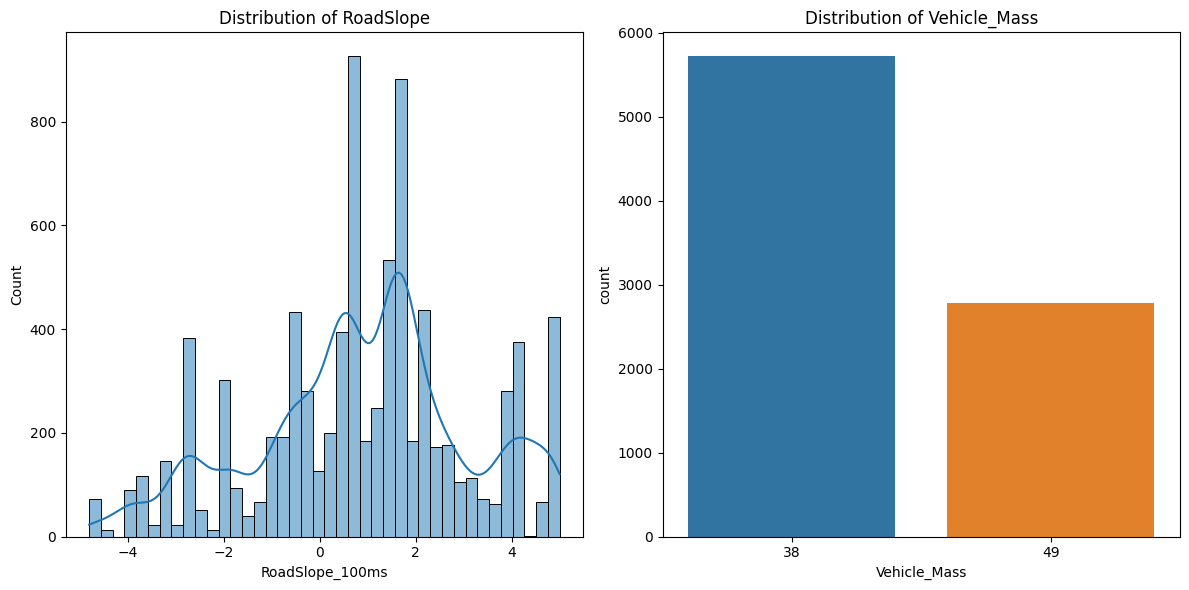
\includegraphics[width=\textwidth, height=0.3\textheight]{Distribution.png}
    \label{fig:roadslopedistribution}
\end{figure*}



\section{Data Preprocessing}
Having identified outliers, correlations, and distributions in the previous step, this section focuses on optimizing the dataset for the task. 
\subsection{Feature Engineering and Reformatting}
\begin{itemize}
\item Irrelevant constant features (`\textbf{CoVeh\_trqAcs\_100ms}`, `\textbf{Com\_rTSC1VRVCURtdrTq}`, `\textbf{Clth\_st`}, `\textbf{CoEng\_st}`, `\textbf{Com\_rTSC1VRRDTrqReq}`) are dropped as they provide no discriminatory information to distinguish between different instances. . 

\item The `\textbf{Vehicle\_Mass}`' column is reformatted to binary encoding for classification.


\end{itemize}

We create a new feature `\textbf{Combined\_VehV\_RngMod}` by combining '\textbf{RngMod\_trqCrSmin}' and '\textbf{VehV\_v}' using formula \ref{eq:1}. This combination is motivated by the strong negative correlation of $-0.63$ observed between these two variables.

\begin{equation} \label{eq:1}
    \hspace{-1em} Combined\_VehV\_RngMod = \dfrac{RngMod\_trqCrSmin\_100ms}{VehV\_v\_100ms}
\end{equation}

\subsection{Task-specific Dataset Splitting}
We initiate the dataset split into features and targets for both the regression and classification tasks, employing the same feature set for both predictions. 

However, we also introduce an alternative `\textbf{MultiTask}` approach. In this strategy, we utilize the predicted vehicle mass values to augment the prediction of road slope. \\

\noindent \textbf{Train-Dev-Test Splitting} \hspace{0.2em} The dataset is partitioned into training, development, and test sets for both regression and classification tasks. The distribution of the dataset across these sets is as follows:

\begin{itemize}
    \item Training Set: 70\%
    \item Development Set: 15\%
    \item Test Set: 15\%
\end{itemize}

\subsection{Feature Scaling}
As we observed numerous outliers in various features (Figure \ref{boxplot}). We address this problem by applying \href{https://scikit-learn.org/stable/modules/generated/sklearn.preprocessing.RobustScaler.html}{Robust scaling} to the features to ensure their uniformity across different scales. 

I also experimented with alternative scaling methods to assess their impact on the overall model performance. The evaluation results are presented in Table \ref{tab:model_performance}.

\begin{table}[h]
    \centering
    \caption{Model Performance with Different Scaling Methods}
    \begin{tabular}{lcc}
    \toprule
    \textbf{Scaling Method} & \textbf{Public Sets} & \textbf{Private Sets} \\
    \midrule
    RobustScaler & 88.03 & 86.63 \\
    StandardScaler & 87.79 & 85.26 \\
    MinMaxScaler & 83.66 & - \\
    MaxAbsScaler & 83.66 & - \\
    Normalizer & 65.83 & - \\
    PowerTransformer & 85.87 & - \\
    QuantileTransformer & 85.33 & - \\
    \bottomrule
    \end{tabular}
    \begin{flushleft}
        \small\textit{Note: Due to limited submit attempts for private sets, evaluation was performed with only two scalers.}
        \end{flushleft}
    \label{tab:model_performance}
    \end{table}
    
\section{Models Selection}
As mentioned above, we will use 2 separate models to address the distinct tasks at hand.
\subsection{Vehicle Mass Classifier Task}\label{task:classifier}



The objective of this task is to train a classifier to categorize a vehicle's mass into two classes: 38 t or 49 t. \\
\noindent \textbf{Random Forest Classifier} \hspace{0.2em} An ensemble learning algorithm that operates by constructing a multitude of decision trees during training and outputting the mode of the classes for classification tasks.


\begin{itemize}
\item Each decision tree in the forest is trained on a random subset of the training data and provides an independent prediction
\item The final classification result is determined by aggregating the predictions from all the individual trees.
\end{itemize}

In addition to the Random Forest classifier, we explored various other classifiers before selecting the final model. The experimentation involved evaluating different algorithms to assess their performance on the Vehicle Mass Classification task. 

\begin{table}[ht]
    \centering
    \caption{G-mean Scores for Vehicle Mass Classification Models}
    \begin{tabular}{lcc}
    \toprule
    \textbf{Classifier} & \textbf{Public Sets} & \textbf{Private Sets} \\
    \midrule
    SVC & 0.9959 & - \\
    Logistic Regression & 0.9748 & - \\
    Decision Tree Classification & 0.9977 & 0.9945 \\
    Random Forest Classification & 0.9988 & 0.9984 \\
    \bottomrule
    \end{tabular}
    \begin{flushleft}
        \small\textit{Note: Due to limited submit attempts for private sets, evaluation was performed with only two best classifiers.}
        \end{flushleft}
    \label{tab:gmean-scores}
\end{table}
    


\subsection{Road Slope Regression Task}
In this task, the goal is to predict the road slope based on the given features. We'll assess the performance of selected models, including KNN Regressor, to achieve accurate predictions.

\noindent \textbf{KNN Regressor} \hspace{0.2em} Predicts the target variable by considering the average or weighted average of the k-nearest data points in the feature space.

The choice of the hyperparameter \texttt{n\_neighbors} in KNN Regressor is crucial, as it determines the number of neighbors that contribute to the prediction. This parameter needs to be carefully tuned for optimal performance.

Figure \ref{fig:different_k_results} shows the experimental results conducted with different values of \texttt{n\_neighbors}.


\begin{figure}[h]
    \centering
    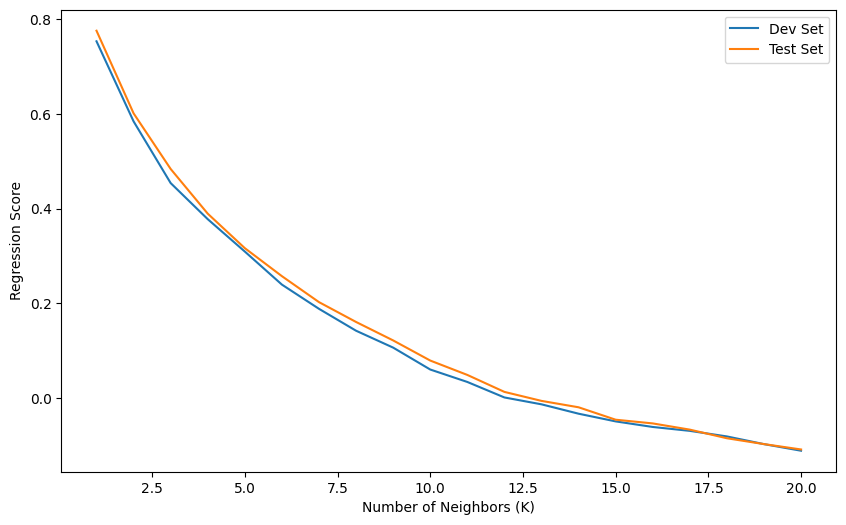
\includegraphics[width=0.5\textwidth]{k_regression_score.png}
    \caption{Regression Performance vs. Number of Neighbors (K)}
    \label{fig:different_k_results}
\end{figure}


In addition to the KNN Regressor, I also evaluated various regression models, from basic ones like SVR, and Bagging, to more complex techniques such as Gradient Boosting and XGBoost.


\begin{figure}[h]
    \centering
    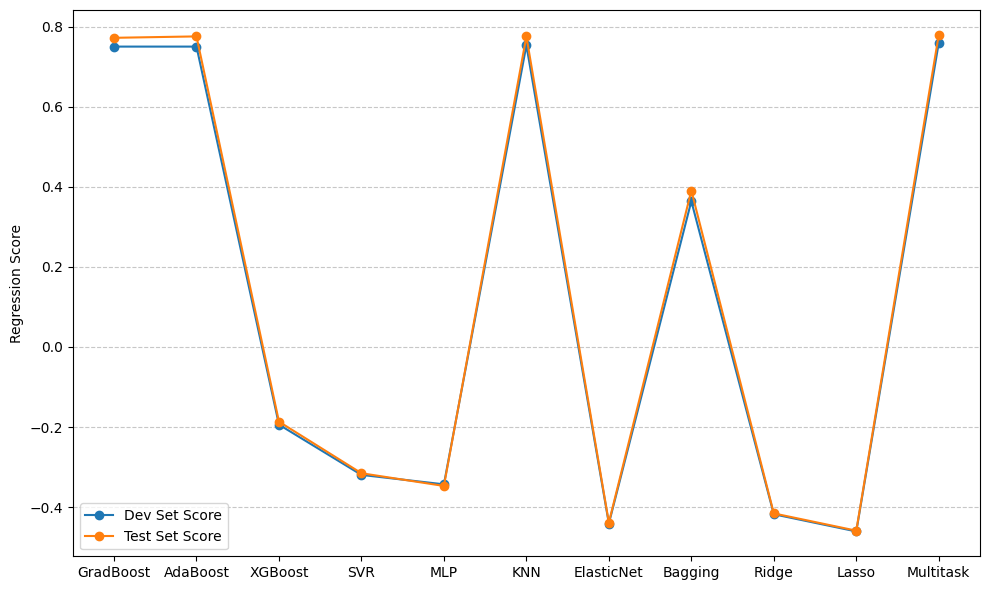
\includegraphics[width=0.5\textwidth]{regression_score.png}
    \caption{Comparison of Models Performance on Dev and Test Sets}
    \label{fig:regression_score}
\end{figure}

Among the regression models, Gradient Boosting, AdaBoost, and K-Nearest Neighbors (KNN) show promising results on both development and test sets. Gradient Boosting and AdaBoost consistently achieve positive scores, indicating strong generalization capabilities. However, in the private test, KNN (\texttt{n\_neighbors} = 1) with tuned parameters outperforms these boosting algorithms


\subsection{MultiTask Approach}
In Figure \ref{fig:regression_score}, the MultiTask approach exhibits competitive performance on both the development and test sets, showcasing results slightly better than KNN. Notably, this approach demonstrates effectiveness in the private test as well.

The concept behind this approach involves utilizing the predicted value of `\textbf{Vehicle\_mass}`', given its high G-score (above 0.998), as an input to predict the road slope.

\section{Evaluation}
Lastly, we will evaluate the performance of the two selected models, \textbf{RandomForest Classifier} and \textbf{KNN Regressor}, on both the public and private contest datasets.


\begin{table}[h]
    \centering
    \renewcommand{\arraystretch}{1.3}  % Increase row spacing
    \begin{tabular}{l@{\hspace{0.6cm}}ccc}  % Increase column spacing
        \toprule
        & \multicolumn{2}{c@{\hspace{0.6cm}}}{Public Set} & \multirow{2}{*}{Private Set} \\
        \cmidrule{2-3}
        & Dev & Test & \\
        \midrule
        Classification Task & 0.999 & 1.000 & 0.998 \\
        Regression Task & 0.754 & 0.776 & 0.795 \\
        \midrule
        Overall Score & 0.840 & 0.854 &  0.866 \\
        \bottomrule
        \vspace{0.5em}
    \end{tabular}
    \caption{Performance Scores on Public and Private Sets}

    \begin{equation*}
        OverallScore = 0.35 \times classification + 0.65 \times regression
    \end{equation*}
    \begin{flushleft}
        \small\textit{Note: The classification performance is evaluated using the G-mean score, and the regression score is defined by the contest.}
        \end{flushleft}

        
    \label{tab:evaluation}
\end{table}

This approach achieved the \textbf{1st} place on both the public test and private test of the course contest with scores of \textbf{199.86} and \textbf{86.63}, respectively. You can find the notebook, submission source code, and model parameters on \href{https://github.com/Dev-Aligator/UIT/tree/master/CS116.O11.KHCL/FinalProject}{GitHub}."


\end{document}
